\chapter{Manufacturing of Planar Detectors}
The manufacturing process of a planar HPGe detector begins with a slice from a crystal boule that has been tested for quality and is know to be detector grade.
Typical boules slices are solid discs that can range from a few millimeters up to several centimeters in thickness and 5+ centimeters in diameter.
This large size allows for several detector samples to be cut from each slice so careful geometry considerations are important in order to minimize wasted material.
The goal is for the detector sample to look approximately like figure \ref{fig:dummydet} which is an example of a planar detector with so called top hat geometry.
\begin{figure}[htpb]
\centering
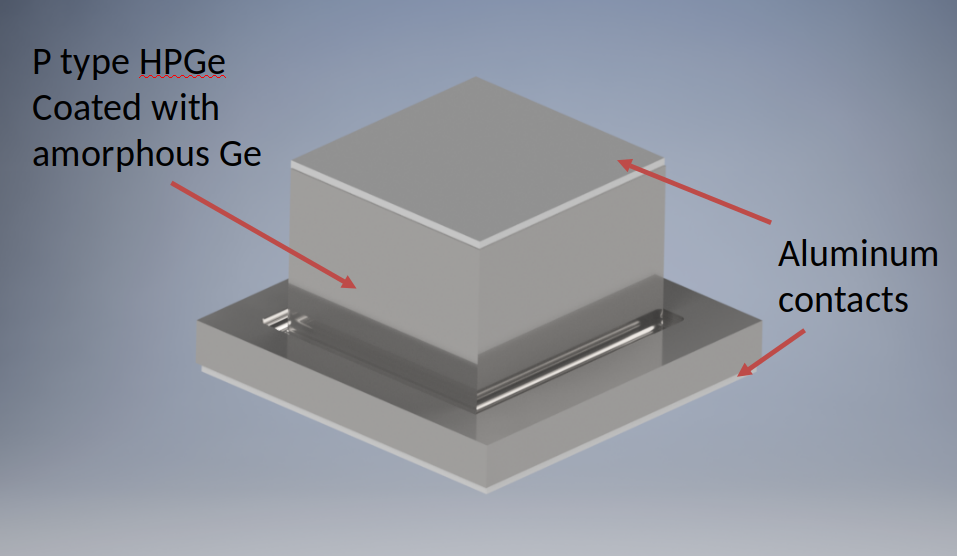
\includegraphics[width=0.5\textwidth]{dummy-det}
\caption{Example detector geometry with four wings}
\label{fig:dummydet}
\end{figure}
The brims of the hat are called wings and serve as a dead area of the detector for handling during the manufacturing process.
The detector is not required to be perfectly square to work so length and width can vary within a few centimeters.
What is of importance are the overall thickness and that the top and bottom faces are parallel.
Due to the relatively long mean free path of gamma rays in germanium, a detector should aim to be at least one centimeter thick.

Once considerations for geometry have been made, the detector manufacturing process begins.
To start, the germanium boule slice is cut into several rectangular cubes.
Then, work proceeds using one of the cubes, saving the rest for the next time.
\subsection{Mechanical Processing}

\begin{figure}[htpb]
\centering
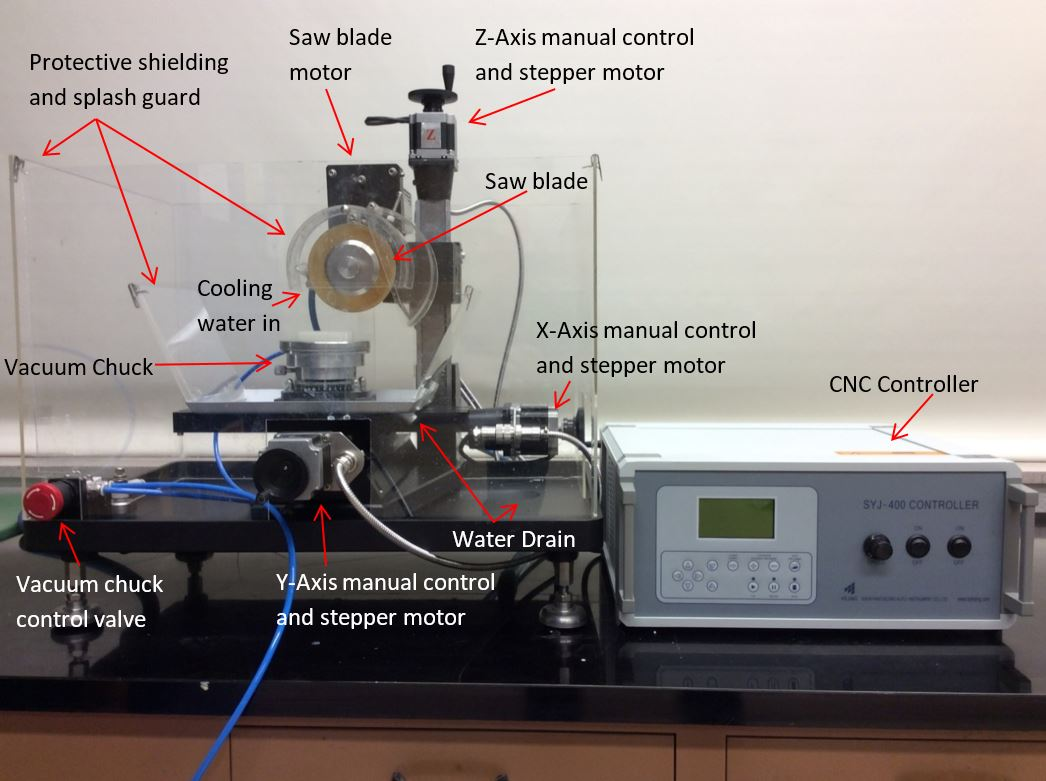
\includegraphics[width=0.5\textwidth]{diamond-saw.jpg}
\caption{The diamond saw used to cut boules into detector samples.}
\label{fig:diamondsaw}
\end{figure}

\begin{figure}[htpb]
\centering
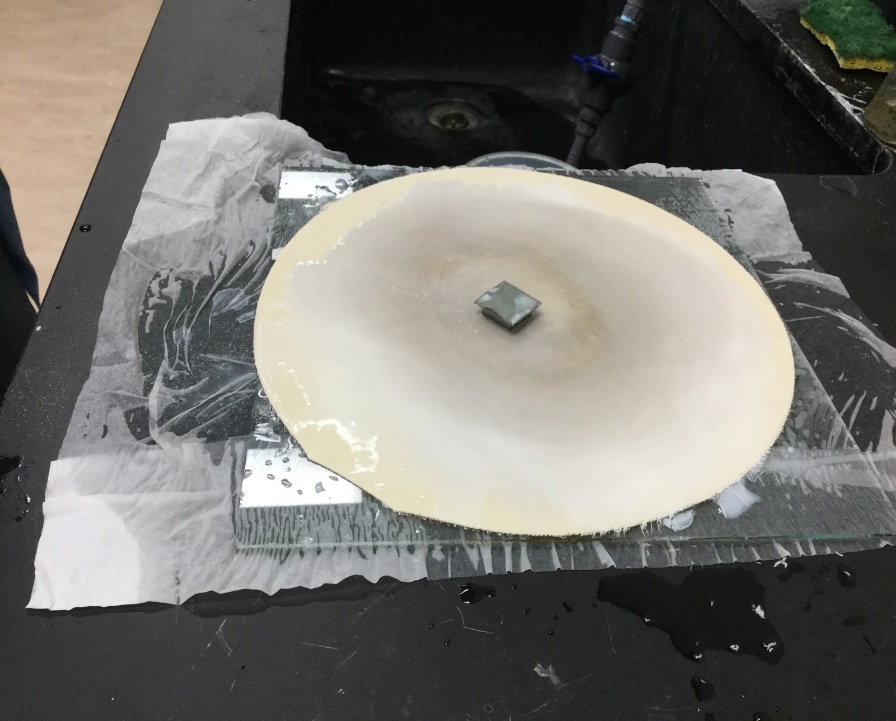
\includegraphics[width=0.5\textwidth]{lapping.jpg}
\caption{An example of lapping the detector sample}
\label{fig:lapping}
\end{figure}

\subsection{Chemical Processing}

\begin{figure}[htpb]
\centering
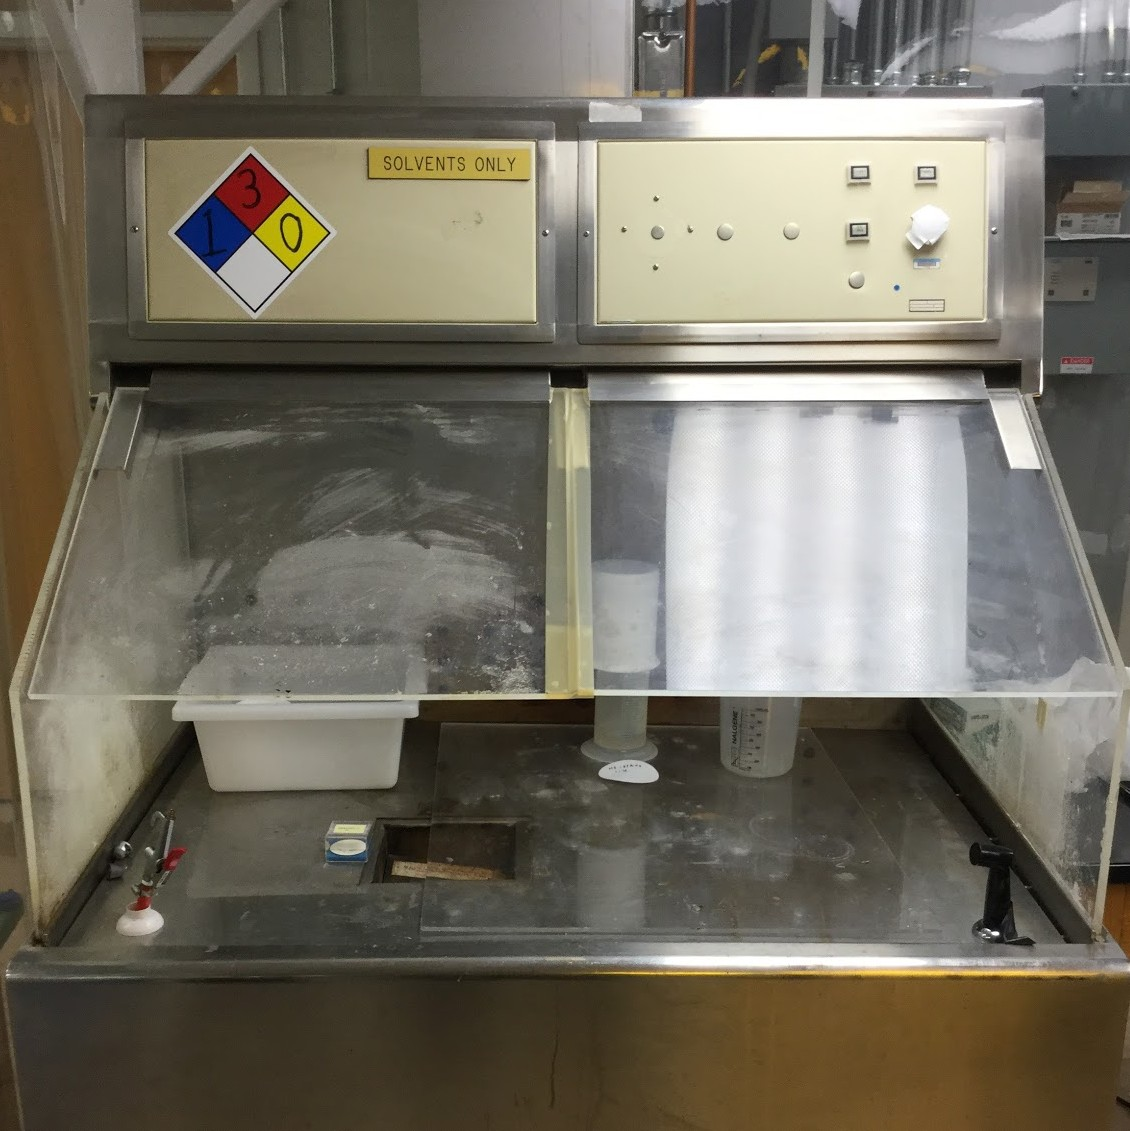
\includegraphics[width=0.5\textwidth]{metal-hood.jpg}
\caption{Metal hood for use with solvents}
\label{fig:metalhood}
\end{figure}


\begin{figure}[htpb]
\centering
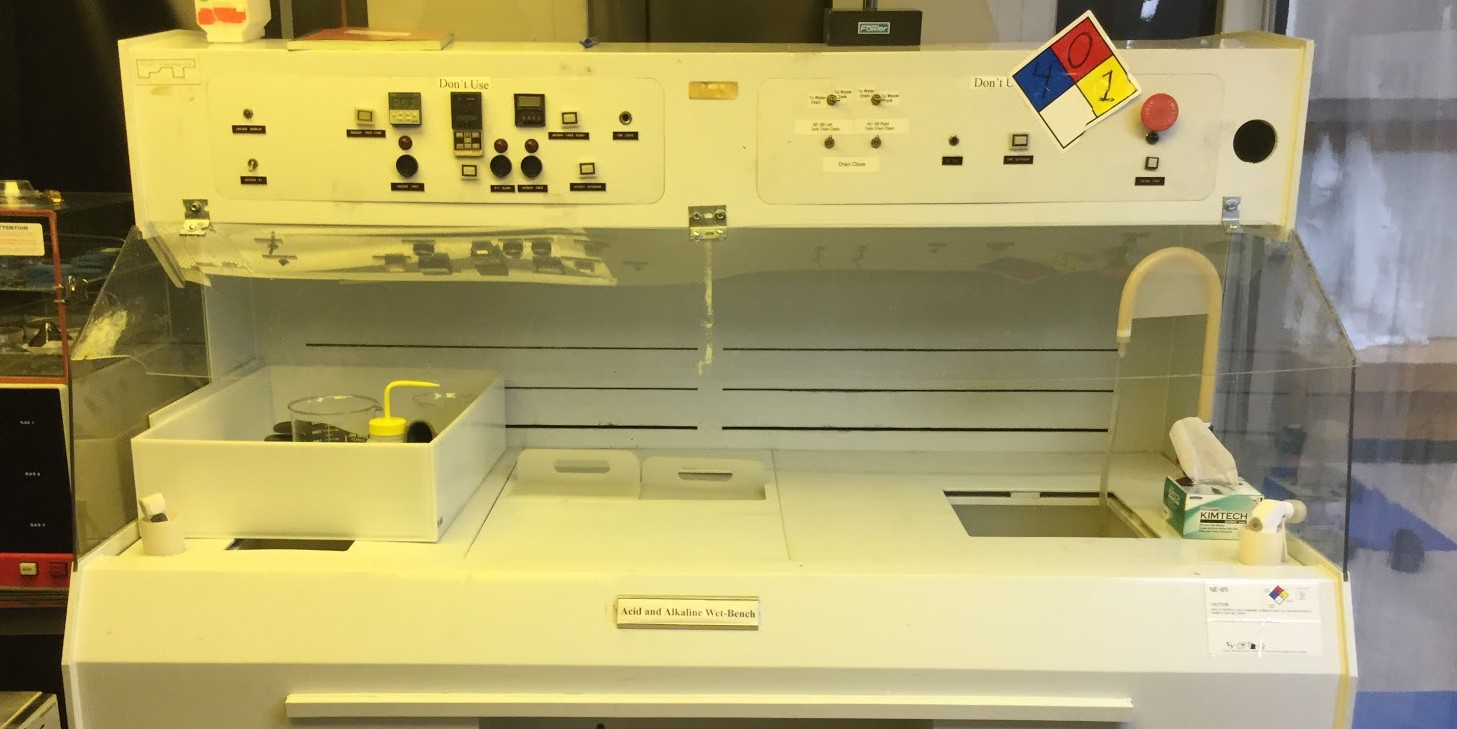
\includegraphics[width=0.5\textwidth]{plastic-hood.jpg}
\caption{Plastic hood for use with acids.}
\label{fig:plastichood}
\end{figure}



\subsection{Amorphous Ge Deposition}

Need information on the working principles of sputtering machine
\subsubsection{Operating Procedure}
The sputtering machine at USD is a Perkin-Elmer 4400 Sputtering System.

The operating procedure for the sputtering machine is complex and care is required to make sure the system maintains working order.
It is a complex system with multiple valves, controls, power supplies, vacuum systems, and pressure monitors that all work in conjunction to deposit a thin layer of amorphous germanium on the detector sample.
One key component of the system is a cryopump that uses pressurized helium gas to quickly vacuum the system to the proper pressure.
The cryopump system can be seen in Figure ~\ref{fig:sput-flow} as blue boxes with labels connected by green lines.
The green lines exchange the helium between the cold head connected to the vacuum chamber and the compressor located in the pump room.
Before the sputtering procedure can begin, the cryopump must be turned on to allow the cold head to cool from room temperature to approximately 20K.
The on\/off switch for the compressor is located on the panel with the other valve toggles and is labeled as "HY-VAC PUMP"

Once the cryopump is cooled down to the proper temperature, the sputtering procedure can begin.
\begin{sidewaysfigure}
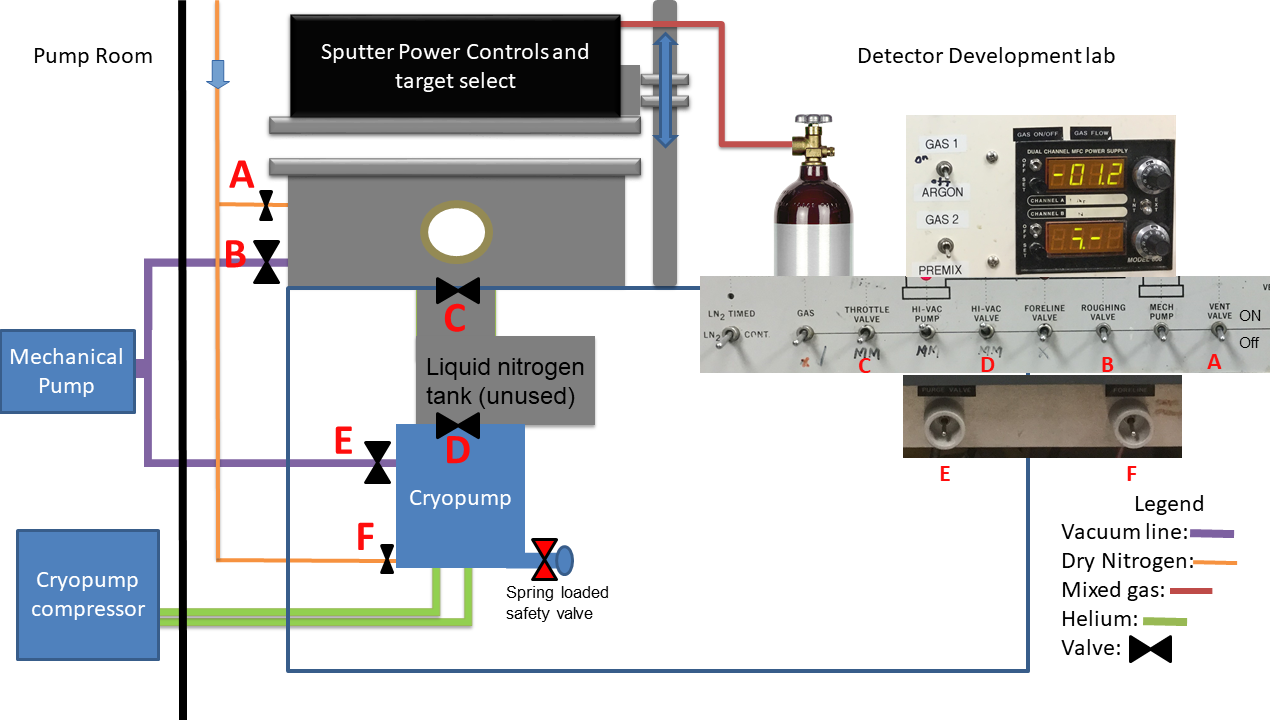
\includegraphics[width=\textwidth]{sput-flow}
\caption{This is a diagram of the Sputtering machine vacuum and gas system. Each valve is connected to a pressurized air line.}
\label{fig:sput-flow}
\end{sidewaysfigure}

\subsection{Aluminum Deposition}

\begin{sidewaysfigure}
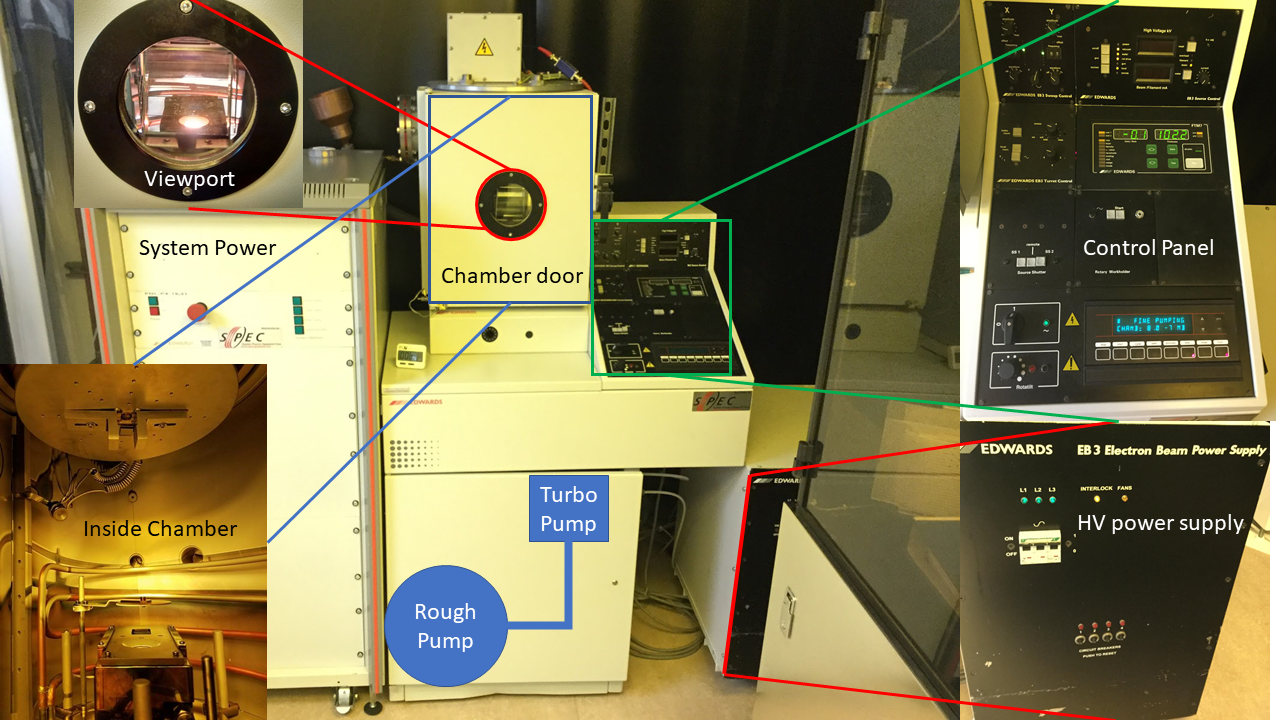
\includegraphics[width=\textwidth]{ebeam-flow}
\caption{This is a diagram of the of the electron beam machine.It is used to deposit aluminum onto the detector sample.}
\label{fig:ebeam-flow}
\end{sidewaysfigure}


\subsection{Final Steps}
